\subsection*{\Large Общая характеристика работы}
\fontsize{14pt}{15pt}\selectfont


\textbf{Актуальность темы исследования.}
Популярность и стремительное развитие систем электронного обучения и платформ для массовых открытых онлайн-курсов MOOC (Massive Open Online Course) в последнее время привели к появлению огромного количества образовательных ресурсов, открытых, но практически никак не связанных между собой. Так крупнейший проект в области MOOC - Coursera насчитывает более 1000 онлайн-курсов, предоставленных более чем 100 университетами и организациями. Другими крупными MOOC порталами являются проекты EdX и Udacity, суммарная аудитория которых превышает 4 миллиона пользователей. В России проект <<ИНТУИТ>> позволяет пользователям бесплатно проходить обучение по образовательным программам, многие из которых касаются информационных технологий. Проект <<ИНТУИТ>> предоставляет пользователям более 800 онлайн-курсов. Проект <<Лекториум>> занимается созданием и размещением открытых учебных курсов в формате видеолекций. Курсы проекта подготовлены ведущими ВУЗами и организациями России. Всего в проекте насчитывается более 4000 часов видеолекций. Отдельный вклад в увеличение количества образовательных ресурсов в сети Интернет внесли электронные библиотеки. Так Британская Библиотека предоставляет информацию о более чем 3,5 миллионах публикаций, книг и монографий в формате открытых данных с помощью проекта BNB (British National Bibliography). 

В области разработки систем обучения и автоматизации образовательных процессов возникает необходимость в сборе, агрегации, гармонизации и повторном использовании учебных материалов различных образовательных ресурсов в контексте одной системы электронного обучения. В настоящее время повторное использование учебных материалов сетевых образовательных ресурсов является одним из наиболее перспективных подходов для разработки систем электронного обучения. Разработка методик агрегации данных позволит создавать распределенные системы электронного обучения использующие учебные материалы из различных образовательных ресурсов университетов, библиотек и организаций.

Одним из методов реализации повторного использования учебных материалов в системах электронного обучения является применение семантических технологий. Технологии семантических сетей (Semantic Web) и связанных данных (Linked Data) позволяют системам обмениваться данными в сети с использованием онтологий и уникальных идентификаторов ресурсов URI (Uniform Resource Identifier). Системы, используя данные технологии, могут интегрировать и адаптировать данные из сторонних источников. Семантические технологии широко используются в образовательных ресурсах в большинстве развитых стран. Наиболее известным проектом в области связанных данных является инициатива Linked Universities. Linked Universities является альянсом европейских университетов распространяющих свои данные, программы, курсы и учебные материалы в формате Linked Data. Другим успешным примером использования семантических технологий в системе электронного обучения является Open University. Open University является исследовательским университетом электронного обучения с более чем 240 тысячами студентов. Семантические технологии используются в прикладных образовательных системах. Одной из таких систем является система SlideWiki - система управления обучением, позволяющая составлять курсы на основе презентаций. Платформа реализует возможность повторного использования данных созданных курсов при составлении нового учебного курса.

Автоматизация сбора, агрегации и гармонизации учебных материалов сетевых образовательных ресурсов в системе электронного обучения позволяет поддерживать содержание образовательного процесса в актуальном состоянии. Пользователям системы предоставляются как одобренные и проверенные учебные материалы, так и материалы из открытых, общедоступных источников. При росте объемов учебных материалов и автоматизации наполнения системы электронного обучения возникает необходимость в контроле качества и целостности учебных курсов и программ. Семантические технологии позволяют формально описывать структуру и связи объектов образовательного процесса. На основе этих связей может быть разработана методика анализа качества учебного курса. 

Действия студентов в системе электронного обучения могут быть связаны с описанными формально объектами образовательного процесса. Разработка методики анализа деятельности пользователей на основе неявных связей с объектами образовательного процесса позволит преподавателям и авторам курсов получить отклик от студентов. На основе анализа качества, целостности курсов, а так же на основе откликов студентов, авторы курсов и преподаватели могут вносить коррективы в образовательный процесс с целью повышения качества обучения. Аналитическая информация деятельности студентов в системе позволит студентам производить мониторинг процесса обучения.     

\textbf{Целью диссертационной работы} является разработка онтологической модели образовательного ресурса и алгоритмов агрегирования и анализа образовательных данных в системе электронного обучения с использованием семантических технологий. 

Для достижения поставленной цели необходимо было решить следующие \textbf{задачи}:
\begin{enumerate}
 \item Разработать онтологические модели для описания учебных материалов, тестов, предметных областей учебных дисциплин, результатов и процесса обучения студентов, метрик оценки знаний и рейтинга студентов;
 \item Разработать методику автоматического агрегирования образовательных данных в системе электронного обучения с использованием методов естественной обработки языка, логического вывода, технологий Semantic Web и Linked Data;
 \item Разработать метод анализа качества и полноты образовательных материалов, основанный на семантических связях в онтологических моделях;
  \item Разработать новый подход к автоматизированной оценке результатов обучения и построению рейтингов студентов системы электронного обучения с использованием статистических методов и семантических технологий;
  \item Создать программные модули для системы электронного обучения на основе разработанных методов и проанализировать полученные результаты на практике.  
 \end{enumerate}

\textbf{Объектом исследования} является структура и логические отношения между объектами образовательного процесса, предметных областей учебных дисциплин и образовательных ресурсов.  

\textbf{Предметом исследования} является алгоритмическое обеспечение, предназначенное для автоматизации процессов наполнения системы электронного обучения учебными материалами, процессов анализа качества учебных материалов и знаний студентов. 

\textbf{Научная новизна.}
\begin{enumerate}
 \item Впервые разработана онтологическая модель, описывающая образовательный процесс, учебные материалы, предметные области, действия студентов и отношения между данными объектами. 
 \item Впервые разработан метод оценки качества и полноты учебного курса на основе анализа неявных семантических связей.
 \item Впервые предложен подход к автоматизированному анализу знаний и рейтингов студентов системы электронного обучения с использованием статистических методов и семантических технологий.
\end{enumerate}

\textbf{Основные положения, выносимые на защиту.}
\begin{enumerate}
 \item Модульная онтология, описывающая структуру образовательного процесса, структуру предметной области учебной дисциплины, структуру тестов, действия и результаты студентов в системе электронного обучения.
 \item Методика наполнения образовательной онтологии и агрегации учебных материалов в системе электронного обучения.
 \item Метод анализа качества и полноты учебного курса;
 \item Алгоритм анализа знаний и рейтинга студентов системы электронного обучения.
 \end{enumerate}


\textbf{Практическая значимость.}
\begin{enumerate}
 \item Разработанная модульная онтология опубликована в сети с зарегистрированными идентификаторами PURLs (Persistent Uniform Resource Locators) и может быть использована для разработки систем электронного обучения.
 \item Программная реализация системы электронного обучения, использующая разработанные модели и алгоритмы, была внедрена на открытой площадке на кафедре проектирования и безопасности компьютерных систем Университета ИТМО (ecole.ifmo.ru). 
 \item Созданы на основе разработанных моделей и алгоритмов и используются на практике онлайн курсы 
<<Интеллектуальные системы>>, <<Физика>>, <<Теория графов>> и <<Аналитическая геометрия и линейная алгебра>>.
 \end{enumerate}
 
 
%\textbf{Достоверность} изложенных в работе результатов обеспечивается ...


\textbf{Апробация работы.}
Основные результаты диссертационной работы докладывались и обсуждались на следующих конференциях:
International Conference on Knowledge Engineering and Semantic Web (Россия, Санкт-Петербург, 2013),
11th Extended Semantic Web Conference (Греция, Аниссарас, 2014), International Conference on Knowledge Engineering and Semantic Web (Россия, Казань, 2013), The 13th International Semantic Web Conference (Италия, Рива-дель-Гарда, 2014), 16th Conference of Open
Innovations Association FRUCT (Финляндия, Оулу, 2014).

%Диссертационная работа была выполнена при поддержке грантов ...

%\textbf{Личный вклад.} Автор принимал активное участие ...

\textbf{Публикации.} Основные результаты по теме диссертации изложены в ХХ печатных изданиях, Х из которых изданы в журналах, рекомендованных ВАК, ХХ --- в тезисах докладов.

%\underline{\textbf{Объем и структура работы.}} Диссертация состоит из~введения, четырех глав, заключения и~приложения. Полный объем диссертации \textbf{ХХХ}~страниц текста с~\textbf{ХХ}~рисунками и~5~таблицами. Список литературы содержит \textbf{ХХX}~наименование.

%\newpage
\subsection*{\Large Содержание работы}
Во \textbf{введении} обосновывается актуальность исследований, проводимых в рамках данной диссертационной работы, приводится обзор научной литературы по изучаемой проблеме, формулируется цель, ставятся задачи работы, сформулированы научная новизна и практическая значимость представляемой работы.

\textbf{Первая глава} посвящена ...

\textbf{Вторая глава} посвящена исследованию 

\textbf{Третья глава} посвящена разработке онтологической модели для описания учебных материалов и образовательного процесса, исследованию методов автоматического агрегирования образовательных данных и разработке методов и подходов к автоматизированной оценке качества учебных курсов и результатов обучения студентов.  

В результате анализа систем электронного обучения была сформирована общая модель данных в системе. Модель делится на три основных уровня: уровень предметных областей, уровень учебных материалов, уровень деятельности пользователей в системе. Уровни модели связаны друг с другом для обеспечения взаимодействия различных ресурсов системы. Уровень предметных областей является основой модели данных и содержит информацию о предметных областях учебных дисциплин. Сбор данных для этого уровня производится из открытых, опубликованных баз знаний, таксономий и наборов данных. Уровень учебных материалов содержит информацию необходимую для проведения учебного процесса. На данном уровне хранятся данные по образовательным программам, курсам, тестам и медиа-ресурсам. Сбор данных для этого уровня производится из хранилищ университетов, открытых электронных библиотек и медиа-ресурсов. Связывание учебных материалов с предметными терминами и областями производится в полуавтоматическом режиме с использованием алгоритмов обработки естественного языка. Уровень деятельности пользователей в системе содержит результаты обучения студентов и  статистические данные по активности пользователей. Статистика ведется в системе управления обучением LMS(Learning Management System). При ведении статистики используется информация из социальных сетей. Связывание статистики и результатов обучения с учебными материалами происходит в автоматическом режиме алгоритмами LMS. Общая модель данных системы электронного обучения представлена на рисунке \ref{fig:OverallModel}. 

\begin{figure}[ht] 
  \center
  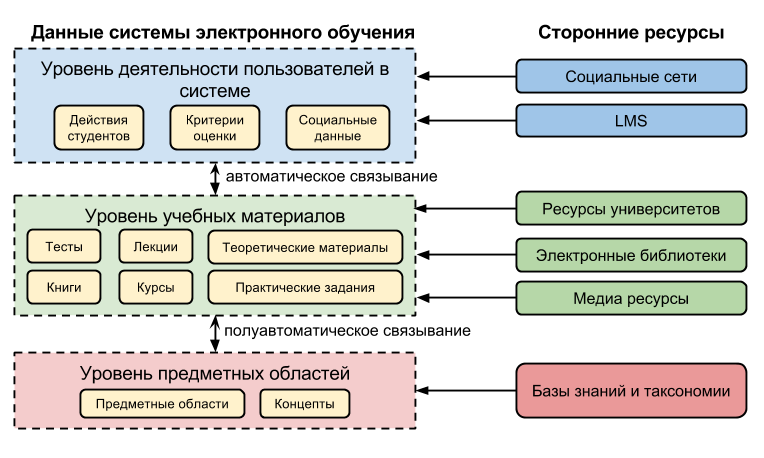
\includegraphics[scale=0.5]{OverallModel}
  \caption{Общая модель данных системы электронного обучения} 
  \label{fig:OverallModel}
\end{figure}

На основе описанной общей модели данных системы была разработана модульная онтология. Модульная онтология состоит из следующих модулей:


\begin{itemize}
\item Модуль учебных материалов - онтология, которая описывает отношения между курсами, модулями, лекциями, тестами, практиками и предметными терминами;
\item Модуль тестов - онтология, которая описывает содержание тестов, вопросы, ответы, варианты тестов;
\item Модуль деятельности и результатов студента в системе обучения - онтология, которая позволяет хранить статистику по действиям студентов в системе и результаты обучения студентов, включая правильные и неправильные ответы на тесты, прохождения лекций и результаты экзаменов.
\item Модуль оценки знаний студентов - онтология, которая позволяет хранить вычисленные автоматически оценки знаний студентов по определенным концептам и предметным областям.
\end{itemize}

Модуль учебных материалов основан на онтологиях верхнего уровня рекомендованных к использованию при описании учебных материалов. При разработке данного модуля использовались онтологии AIISO (The Academic Institution Internal Structure Ontology), BIBO (The Bibliographic Ontology) и MA-ONT (The Ontology for Media Resources). Модуль учебных материалов является связующим звеном для всех модулей разработанной онтологии. Одной из главных особенностей разработанной онтологии является возможность произведения прямого и косвенного междисциплинарного связывания объектов в курсах.   

% Показать пример связывания
% Показать схему онтологии
% Привести выходные данные

В продолжении главы описывается разработанная методика по агрегации и гармонизации учебных материалов в системе электронного обучения. Технологии Semantic Web и Linked Data позволяют использовать онтологии для хранения, сбора и распространения данных. Одним из преимуществ данных технологий является повторное использование данных. В Интернете существует множество открытых источников с данными, при описании которых были использованы онтологии верхнего уровня. Данные источники могут быть использованы для наполнения системы электронного обучения. Для сбора и интеграции данных в системе электронного обучения предлагается использовать провайдеры данных. Провайдеры данных это программные модули  поддерживают автоматическое обновление связных данных из открытых источников, используя определенный алгоритм. Провайдеры позволяют преобразовывать структурированные данных различных форматов в формат RDF. Каждый провайдер обладает своим контекстом для дальнейшего управления собранными данными. В результате исследования был сформирован следующий набор методов агрегации данных:

\begin{itemize}
\item интеграция связанных данных из открытых источников в формате RDF на примере связывания учебных курсов с данными электронной библиотеки BNB;
\item интеграция и преобразование структурированных данных в форматах XML и JSON в формат RDF с использованием отображения на примере адаптации тестов Университета ИТМО;
\item интеграция результатов SPARQL запросов к открытым точкам доступа на примере сбора определений для предметных терминов из электронной энциклопедии DBpedia;
\item интеграция результатов REST запросов с использованием отражения на примере связывания учебных курсов с данными портала учебных изданий Университета ИТМО;
\item применение методов обработки естественного языка для создания дополнительных связей между объектами на примере связывания предметных терминов с заданиями учебных тестов.
\end{itemize}

Особое внимание в главе уделяется применению методов обработки естественного языка для гармонизации объектов в онтологии. Для наполнения онтологий системы можно использовать не только данные внешних источников, но и данные самой системы. Данные хранящиеся в онтологии системы и связанные семантическими связями позволяют создавать новые связи на основе предопределенных правил. Используя методы обработки естественного языка можно извлекать семантические связи из текстовой информации объекта онтологии. В исследовании данные методы использовались для выявления связей между предметными терминами и заданиями теста. В задании в тексте вопроса и его ответов производился поиск предметных терминов. Найденные термины связывались с заданиями теста. Данные связи обозначали использование предметного термина в задании учебного теста и позволяли формально описать содержание задания. 

Для реализации алгоритма связывания заданий тестов и предметных терминов был разработан провайдер данных. Провайдер принимает на вход ссылку на объект курса и производит создание ссылок между заданиями и терминами. Для извлечения терминов была использована лингвистическая платформа NooJ. Общий алгоритм работы провайдера данных представлен на рисунке \ref{fig:NLPAlgo}.

\begin{figure}[ht] 
  \center
  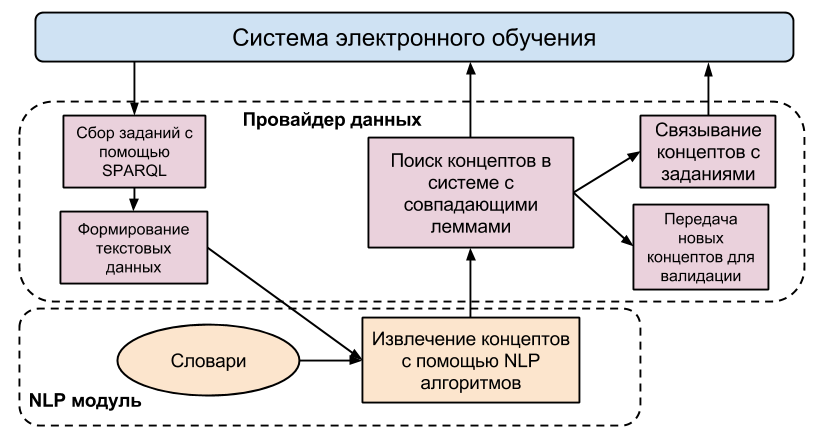
\includegraphics[scale=0.45]{NLPAlgo}
  \caption{Алгоритм работы провайдера извлечения терминов с использованием методов обработки естественного языка} 
  \label{fig:NLPAlgo}
\end{figure}

Алгоритм состоит из следующих шагов:

\begin{itemize}
\item провайдер собирает список заданий курса, используя запросы SPARQL;
\item производится формирование текстовых данных для каждого задания, используя информацию о вопросах и ответах;
\item провайдер данных запускает NLP алгоритмы в платформе NooJ для текстовых данных каждого задания;
\item провайдер формирует список терминов-кандидатов содержащих каноническую форму и набор лемм;
\item производится поиск предметных терминов в системе с совпадающими наборами лемм для дальнейшего связывания с терминами кандидатами;
\item провайдер создает связи между найденными предметными терминами системы и заданиями терминов-кандидатов с помощью объектного свойства <<hasTerm>>.
\end{itemize}


% Можно сократить - убрать
Термины-кандидаты, для которых не были найдены соответствующие предметные термины системы, могут быть записаны в онтологию, как новые предметные термины системы. Перед записью в онтологию провайдер производит проверку термина-кандидата на соответствие предметному термину. Для проверки используются запросы к базе знаний DBpedia. В случае совпадения названия термина-кандидата со свойствами <<rdfs:label>> или <<dbpedia-owl:wikiPageRedirects>> объекта из DBpedia, в онтологии системы создается новый предметный термин на основе термина-кандидата и производится связывание с заданиями теста. При отсутствии совпадений термин-кандидат помечается провайдером данных как ложный термин. При SPARQL запросах к базе знаний DBpedia используется фильтрация по предметным областям и категориям. Данная фильтрация позволяет избежать ошибочных совпадений терминов-кандидатов с терминами из сторонних предметных областей. Для включения нового термина в систему необходима верификация преподавателя или администратора системы. 

Далее в главе описывается разработка методов анализа качества и полноты учебного курса. Метод основан на анализе косвенных связей в онтологии системы. Аналитика формируется из статистических данных, полученных с помощью SPARQL запросов. 

Одним из примеров использования метода является анализ покрытия лекций курса тестами и заданиями. В онтологии системы лекции и тесты связаны с определенным модулем курса. В результате работы алгоритмов по наполнению онтологий лекции и задания тестов могут быть связаны с определенными предметными терминами. Таким образом, происходит косвенное связывание лекций и тестов через предметные термины. Если термин лекции использован в задании теста, он считается покрытым в данном модуле учебного курса.

Другим подходом к анализу учебных материалов является выявление проблемных предметных терминов в модуле учебного курса. Проблемными предметными терминами являются термины, при изучении которых у студентов возникают наибольшие затруднения. Статистика по результатам прохождения студентами тестов, правильные и неправильные ответы на задания связанные с определенными предметными терминами позволяют рассчитать общий рейтинг знания студентами определенного термина. Используя данный рейтинг, преподаватель, может получить список предметных терминов курса, которых студенты знают хуже всего. Это позволит преподавателю вносить коррективы в учебные материалы и учебный процесс. В текущей реализации метода используется упрощенная формула расчета рейтинга проблемного термина. Рейтинг проблемного термина рассчитывается делением количества неправильных ответов на количество правильных ответов на задания связанные с данным термином. Данная формула может быть усовершенствована с помощью включения дополнительных параметров. Рейтинг проблемных терминов для модуля составляется с помощью следующего  SPARQL-запроса:

\begin{verbatim}
    SELECT ?term 
        (count(?correct_answer) AS ?correct_answer_count)
        (count(?answer) AS ?answer_count)
        ((2*?correct_answer_count - ?answer_count) 
            AS ?rank) 
    WHERE{
        ?module learningRu:hasTest ?test  . 
        ?test ifmotest:hasGroupOfTasks 
            ?group_of_tasks .        
        ?group_of_tasks ifmotest:hasTask ?task .      
        ?test_element lres:hasTask ?task .
        ?test_element lres:hasAnswer ?answer .
        ?task learningRu:hasTerm ?term .       
        OPTIONAL { 
            ?task ifmotest:hasCorrectAnswer 
                ?correct_answer
            filter( ?correct_answer = ?answer)
        }         
    }
    GROUP BY ?term 
    ORDER BY ASC(?rank)
\end{verbatim}


Аналитка качества учебного курса состоит из следующей статистической информации:
\begin{itemize}
\item количество покрытых и непокрытых предметных терминов в модуле учебного курса;
\item общий процент покрытия модуля тестами на основе отношения покрытых терминов к общему количеству терминов;
\item облако тегов предметных терминов модуля демонстрирующее качество и степень покрытия каждого термина;
\item список непокрытых терминов модуля, которые были использованы в лекциях, но не были использованы в заданиях тестов;
\item список проблемных предметных терминов с рейтингами в модуле учебного курса;
\item диаграмма отношений между пятью самыми проблемными терминами модуля учебного курса.
\end{itemize}


В конце главы описывается новый подход к автоматизированному анализу знаний и рейтингов студентов системы электронного обучения с использованием статистических методов и семантических технологий. Данный подход позволяет студентам получать информацию о своих знаниях по предметным терминам и предметным областям учебных дисциплин в режиме реального времени. Такая информация может использоваться студентами для выявления пробелов в знаниях и при повторении пройденных учебных материалов. В дальнейшем развитии подхода информация о знаниях и результатах позволит формировать рекомендации для студентов по образовательным программам и исследовательским проектам и лабораториям. Преподаватели смогут использовать информацию о знаниях и результатах студентов во время подготовки к проведению учебного курса и лекций у определенной группы студентов.

Подход основан на семантическом анализе действий студентов в системе электронного обучения в проекции образовательного процесса и учебных материалов. Целью подхода является автоматизированный вывод рейтинга знаний студентом определенной предметной области учебной дисциплины. Рейтинг знания предметной области зависит от рейтингов входящих в нее предметных терминов. Расчет рейтинга знания предметного термина зависит от метрик оценки действий студента в системе. Набор метрик может варьироваться в зависимости от возможных действий студентов в системе, структуры онтологии и необходимой точности вычислений. В предложенном подходе используются метрики: метрика знакомства с термином и метрика проверки знания термина с помощью тестов. Основными шагами расчета рейтинга знания предметной области являются:


\begin{itemize}
\item расчет рейтинга знания предметного термина с учетом метрики знакомства с термином;
\item расчет рейтинга знания предметного термина с учетом метрики проверки знания термина с помощью тестов;
% \item расчет рейтингов знания терминов в контексте прохождения одного теста;
\item расчет суммарного рейтинга знания предметного термина;
\item расчет значения предметного термина в образовательном процессе;
\item расчет рейтинга знаний предметной области с учетом значения предметных терминов в образовательном процессе.
\end{itemize}

Рейтинг знания термина, как и рейтинг знания предметной области, варьируется от 0 до 1. Метрика знакомства с термином является бинарной метрикой и обозначает факт изучения студентом предметного термина с использованием теоретического материала. В разработанном подходе изучением предметного термина является завершение студентом лекции связанной с данным термином в системе электронного обучения. Изучить предметный термин студент может только один раз. В разработанном подходе данная метрика составляет 15\% от общего рейтинга знаний предметного термина.

Метрика проверки знания предметного термина с помощью тестов основана на статистическом анализе правильных и неправильных ответов студента на задания учебных курсов, которые связаны с данным термином. В разработанном подходе данная метрика составляет 85\% от общего рейтинга знаний предметного термина. Метрика рассчитывается как нижняя граница доверительного интервала Вильсона для параметра Бернулли по количеству правильных и неправильных ответов, используя формулу:

$$
    R_t = \frac{p+\frac{1}{2n}z_{1-\alpha/2}^2 \pm z_{1-\alpha/2}\sqrt{\frac{p(1-p)}{n}+\frac{z_{1-\alpha/2}^2}{4n^2}}{} }{1+\frac{1}{n}z_{1-\alpha/2}^2},
$$

где \(z_{1-\alpha/2}\) - квантиль от от \(1-\alpha/2\) стандартного нормального распределения, \(p\) - доля правильных ответов, \(n\) - общее количество ответов. 

Сумма двух полученных метрик для предметного термина в соответствии с их долями является общим рейтингом знания предметного термина. Предметные области и предметные термины в соответствии с разработанной моделью не зависят от учебных материалов и могут повторно использоваться в множестве учебных курсов. Связи между терминами описывающие необходимость одного термина для изучения другого позволяют рассчитать важность предметного термина в образовательном процессе. Чем больше предметных терминов, для изучения которых необходим определенный термин тем выше значение данного термина. При расчете учитывается количество терминов на разных уровнях зависимости. Уровнем зависимости является глубина косвенной зависимости одного термина от другого через набор терминов. Например, на втором уровне зависимости находятся термины, зависимые от предметных терминов зависимых от рассматриваемого предметного термина. Значение термина рассчитывается с использованием трех уровней зависимости по формуле: 

$$
    W_t = \frac{1}{e}+\sum_{k=1}^{3}\frac{n_k}{e^k}, 
$$

где \(n\) - количество терминов связанных с данным термином на каждом уровне зависимости, \(k\) - номер зависимого уровня, \( \frac{1}{e} \) - константное значение термина. 

Итоговый рейтинг знания студентом предметной области учебной дисциплины рассчитывается как сумма рейтингов предметных терминов, входящих в предметную область. При расчете необходимо учитывать относительное значение термина в предметной области. Для этого необходимо рассчитать суммарное значение предметной области, используя формулу:

$$  
    W_f = \sum_{n=1}^{\infty}W_t,
$$

где \(W_t\) - значение предметного термина, \(n\) - количество терминов в предметной области.

Относительное значение термина в предметной области рассчитывается по формуле:

$$
    D_t = \frac{W_t}{W_f},
$$

где \(W_t\) - значение термина, \(W_f\) - значение предметной области.

Рейтинг предметной области является суммой рейтингов предметных терминов в соответствии с их относительными значениями:

$$
    R_f = \sum_{n=1}^{\infty} R_tD_t,
$$
где \(R_t\) рейтинг термина, \(D_t\) - относительное значение термина в предметной области.

Представленный подход позволяет производить автоматизированную оценку знания студентами предметных областей. Поддержка набора метрик позволяет системе варьировать алгоритмы расчета оценки, добавляя, изменяя и удаляя необходимые метрики. Помимо оценки предметных областей данный подход можно применять к любым объектам образовательного процесса напрямую или косвенно связанным с предметными терминами. Подход позволяет производить оценку учебных курсов и специальностей.  

В \textbf{четвертой главе} приведено описание архитектуры и особенности реализации программных модулей для системы электронного обучения. Также в главе описаны основные результаты исследований по разработанным методикам.

На основе разработанных моделей и методик были реализованы программные модули, которые в своей комбинации формирую ядро системы электронного обучения ECOLE (Enhanced Course Ontology for Linked Education). Сервер системы ECOLE реализован на языке Java и основан на платформе Information Workbench. Платформа Information Workbench предоставляет функционал для работы с открытыми связными данными. Редактирование и управление RDF данными системы реализовано с использованием платформы OpenRDF Sesame. Сервер системы ECOLE предоставляет открытую точку доступа для SPARQL запросов. 

Внешним интерфейсом системы дистанционного обучения ECOLE является система управления образованием Learning Management System (LMS). LMS обладает локальным хранилищем и производит управление пользовательскими данными, настройками и результатами обучения студентов. В LMS реализованы модули для отображения видео-лекций, слайдов, тестов и практических заданий. Внешний интерфейс получает с сервера данные по учебным материалам и отношения между объектами курса с помощью запросов к открытой точке доступа SPARQL. Персональные данные пользователей и настройки LMS хранятся в локальной памяти внешнего интерфейса. С помощью алгоритмов LMS производится сбор статистических данных по действиям студентов в системе и запись их в онтологии на сервере системы. LMS реализована на языке Python с использованием Django Web Framework. Общая архитектура системы электронного обучения ECOLE представлена на рисунке \ref{fig:OverallArch}.


\begin{figure}[ht] 
  \center
  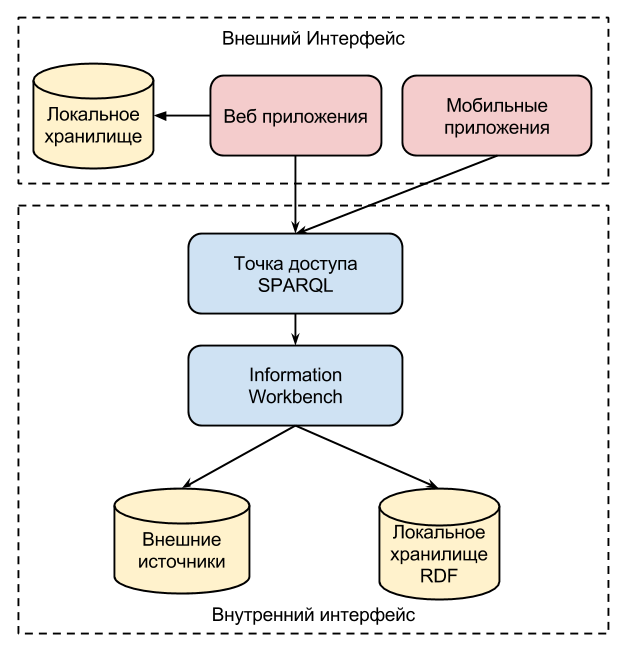
\includegraphics[scale=0.45]{OverallArch}
  \caption{Общая архитектура системы электронного обучения ECOLE} 
  \label{fig:OverallArch}
\end{figure}


После прохождения теста система предоставляет студенту информацию о количестве и доле правильных ответов на задания теста и список предметных терминов для повторения. На основе разработанных методов система расчитывает рейтинг знаний предметных терминов и областей.   
% Вставить скриншоты рейтинов (список терминов)


% Написать про результаты
% Количество агрегированных объектов
% Результаты по NLP
% Результаты по качеству курсов и рейтингам

В \textbf{заключении} приведены основные результаты работы, которые заключаются в следующем:
\begin{enumerate}
 \item Разработаны онтологические модели для описания учебных материалов, тестов, предметных областей учебных дисциплин, результатов и процесса обучения студентов, метрик оценки знаний и рейтинга студентов;
 \item Разработана методика автоматического агрегирования образовательных данных в системе электронного обучения с использованием методов естественной обработки языка, логического вывода, технологий Semantic Web и Linked Data;
 \item Разработан метод анализа качества и полноты образовательных материалов, основанный на разборе семантических связей между объектами системы;
  \item Разработан новый подход к автоматизированному анализу знаний и рейтингов студентов системы электронного обучения с использованием статистических методов и семантических технологий;
  \item Созданы программные модули для системы электронного обучения на основе разработанных методов и подходов;
  \item Произведен анализ результатов работы методов и подходов, полученных при прохождении группой студентов учебного курса <<Интеллектуальные системы>>.
  \end{enumerate}



%\newpage
\renewcommand{\refname}{\Large Публикации автора по теме диссертации}
\nocite{*}
\bibliography{biblio}